\documentclass{beamer}
\setbeamercovered{}

\usepackage{bookman}
\usepackage{newtxtext}
\usepackage{amssymb}
\usepackage{amsmath}
\usepackage{amsfonts}
\usepackage{mathrsfs}
\usepackage{mathtools}
\usepackage{hyperref}
\usepackage{pifont}
\usepackage{tasks}
\usepackage{systeme}
\usepackage{subcaption}
\usepackage{bm} % Bold
\usepackage{bbm} % Can use \mathbbm{1}
\usepackage{ifthen} % Use if then else
\usepackage{shuffle} % Use shuffle product
\usepackage{minted} % For listing codes
\usepackage{tikz}
\usetikzlibrary{calc}
\usepackage{pgfplots}

\makeatletter
\newcommand*{\Relbarfill@}{\arrowfill@\Relbar\Relbar\Relbar}
% \newcommand*{\relbarfill@}{\arrowfill@\relbar-\relbar}
\newcommand*{\xequal}[2][]{\ext@arrow 0055\Relbarfill@{#1}{#2}}
% \newcommand*{\xdash}[2][]{\ext@arrow 0055\relbarfill@{#1}{#2}}
\makeatother

\newlength{\simlength}

\newcommand{\xsim}[1]{
\settowidth{\simlength}{$#1$}
\mathrel{\overset{#1}{\resizebox{\simlength}{\height}{\sim}}}
}

\mode<presentation> {
    \usetheme{Madrid}
    \usecolortheme{beaver}
    \usefonttheme{professionalfonts} 
    \setbeamertemplate{navigation symbols}{}
    \setbeamertemplate{caption}[numbered]
}

\theoremstyle{definition}
\newtheorem{proposition}[theorem]{Proposition}
\newtheorem{construction}[theorem]{Construction}
\newtheorem{deduction}[theorem]{Deduction}
\newtheorem{exercise}[theorem]{Exercise}
\newtheorem{conjecture}[theorem]{Conjecture}

\theoremstyle{remark}
\newtheorem*{remark}{Remark}
\newtheorem*{recall}{Recall}
\newtheorem*{question}{Question}
\newtheorem*{answer}{Answer}

\newcounter{saveenumi}
\newcommand{\seti}{\setcounter{saveenumi}{\value{enumi}}}
\newcommand{\conti}{\setcounter{enumi}{\value{saveenumi}}}
\DeclareMathOperator{\Span}{Span}
\DeclareMathOperator{\Vol}{Vol}
\resetcounteronoverlays{saveenumi}

\AtBeginSection[]{
    \begin{frame}
    \centering
    \begin{beamercolorbox}[center, shadow=true, rounded=true]{title}
    \usebeamerfont{title}\insertsectionhead\par%
    \end{beamercolorbox}
    \end{frame}
}

\title{MATH240 - Introduction to Linear Algebra}
\author{Haoran Li}
\institute[UMD]{University of Maryland, College Park}
\date{Summer 2024}


\begin{document}

\maketitle

\section{Lecture 8 - Determinant}

\begin{frame}[t]
\begin{definition}
We say a square matrix $A$ is \textcolor{blue}{upper triangular}\index{upper triangular} if it only has zeros to the left of the diagonal
\[
\begin{bmatrix}
*&*&*&*&*&*\\
0&*&*&*&*&*\\
0&0&*&*&*&*\\
0&0&0&*&*&*\\
0&0&0&0&*&*\\
0&0&0&0&0&*\\
\end{bmatrix}
\]\pause
$A$ is \textcolor{blue}{lower triangular}\index{lower triangular} if it only has zeros to the right of the diagonal
\[
\begin{bmatrix}
*&0&0&0&0&0\\
*&*&0&0&0&0\\
*&*&*&0&0&0\\
*&*&*&*&0&0\\
*&*&*&*&*&0\\
*&*&*&*&*&*\\
\end{bmatrix}
\]
\end{definition}
\end{frame}

\begin{frame}[t]
\begin{definition}
$A$ is \textcolor{blue}{diagonal} if $A$ only has nonzero entries on the diagonal
\[
\begin{bmatrix}
*&0&0&0&0&0\\
0&*&0&0&0&0\\
0&0&*&0&0&0\\
0&0&0&*&0&0\\
0&0&0&0&*&0\\
0&0&0&0&0&*
\end{bmatrix}
\]\pause
A diagonal matrix is both upper triangular and lower triangular
\end{definition}
\end{frame}

\begin{frame}[t]
Now let's introduce \textcolor{blue}{determinants} \index{determinant}(\textcolor{red}{ONLY for square matrices!!!}). Consider the parallelepiped $P$ with edges $\mathbf a_1,\cdots,\mathbf a_n$ in $\mathbb R^n$. We would like the following geometric definition of determinants.
\pause
\begin{definition}
The determinant of $A=\begin{bmatrix}
\mathbf a_1&\cdots&\mathbf a_n
\end{bmatrix}$ (Usually denoted $\det A$ or $|A|=\left|\begin{matrix}\mathbf a_1&\cdots&\mathbf a_n\end{matrix}\right|$, replacing brackets with vertical lines) as \textit{signed} volumes of $P$ . Therefore we have $\Vol(P)=|\det A|$, i.e. actual volume is the absolute value of the determinant.
\end{definition}
\pause
\begin{example}[$n=1$]
Suppose $A=[a]$ is a 1 by 1 matrix, then $\det A$ is the signed length of $a\in\mathbb R^1$, which is $a$ itself! Namely $\det A=a$.
\begin{center}
\begin{tikzpicture}
\draw[->] (-2,0)--(2,0);
\filldraw (0,0) circle (0.02);
\draw[->, thick] (0,0)--(1,0) node[below] {$\mathbf a$};
\end{tikzpicture}
\end{center}
\end{example}
\end{frame}

\begin{frame}[t]
\begin{example}[$n=2$]
Suppose $A=\begin{bmatrix}\mathbf a_1&\mathbf a_2\end{bmatrix}$ is a 2 by 2 matrix. $\det A$ is the actual positive area of the parallelogram if $\mathbf a_1$ turns counter-clockwise to $\mathbf a_2$, otherwise the negative area.
\begin{center}
\begin{tikzpicture}[scale=2]
\begin{scope}[xshift=-1cm]
\coordinate (o) at (0,0);
\coordinate (a1) at (1,0);
\coordinate (a2) at ($cos(60)*(1.2,0)+sin(60)*(0,1.2)$);
\draw[->, thick] (o)--(a1);
\draw[->, thick] (o)--(a2);
\draw[dashed] (a1)--($(a1)+(a2)$)--(a2);
\draw[->] (0.4,0) arc (0:60:0.4);
\node at (a1)[right] {$\mathbf a_1$};
\node at (a2)[above] {$\mathbf a_2$};
\node at ($0.5*(a1)+0.5*(a2)$){$+$};
\end{scope}
\begin{scope}[xshift=1cm]
\coordinate (o) at (0,0);
\coordinate (a2) at (1,0);
\coordinate (a1) at ($cos(60)*(1.2,0)+sin(60)*(0,1.2)$);
\draw[->, thick] (o)--(a1);
\draw[->, thick] (o)--(a2);
\draw[dashed] (a1)--($(a1)+(a2)$)--(a2);
\draw[<-] (0.4,0) arc (0:60:0.4);
\node at (a1)[above] {$\mathbf a_1$};
\node at (a2)[right] {$\mathbf a_2$};
\node at ($0.5*(a1)+0.5*(a2)$){$-$};
\end{scope}
\end{tikzpicture}
\end{center}
\end{example}
\pause
\begin{example}[$n=3$]
Suppose $A=\begin{bmatrix}\mathbf a_1&\mathbf a_2&\mathbf a_3\end{bmatrix}$ is a 3 by 3 matrix. To decide the sign of the volume of the parallelepiped, we follow the \textcolor{blue}{right-hand rule}.
\end{example}
\end{frame}

\begin{frame}[t]
\begin{center}
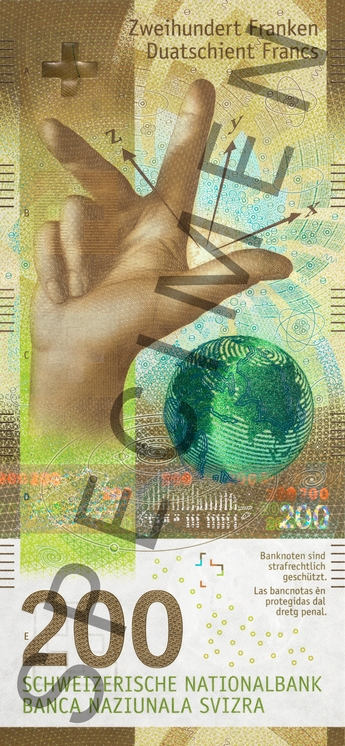
\includegraphics[scale=.33]{righthandrule.jpg}
\begin{tikzpicture}[scale=0.75]
\def\xangle{-80}
\def\yangle{0}
\def\zangle{-5}
\foreach \u/\v/\w/\U/\V/\W/\xshift/\yshift/\sign in {
a1/a2/a3/{a_1}/{a_2}/{a_3}/-1/2/+,
a1/a3/a2/{a_1}/{a_3}/{a_2}/1/2/-,
a2/a1/a3/{a_2}/{a_1}/{a_3}/-1/0/-,
a2/a3/a1/{a_2}/{a_3}/{a_1}/1/0/+,
a3/a1/a2/{a_3}/{a_1}/{a_2}/-1/-2/+,
a3/a2/a1/{a_3}/{a_2}/{a_1}/1/-2/-
}{
\begin{scope}[scale=2,rotate around x=\xangle,rotate around y=\yangle,rotate around z=\zangle,xshift=\xshift cm,yshift=\yshift cm]
\coordinate (o) at (0,0,0);
\coordinate (e1) at (1,0,0);
\coordinate (e2) at (0,1,0);
\coordinate (e3) at (0,0,1);
\coordinate (\u) at (e1);
\coordinate (\v) at (e2);
\coordinate (\w) at (e3);
\draw[->, thick] (o)--(\u)node[below right]{$\mathbf \U$};
\draw[->, thick, dashed] (o)--(\v)node[above right]{$\mathbf \V$};
\draw[->, thick] (o)--(\w)node[left]{$\mathbf \W$};
\draw (e1)--($(e1)+(e3)$)--($(e1)+(e2)+(e3)$)--($(e1)+(e2)$)--cycle;
\draw (e3)--($(e1)+(e3)$)--($(e1)+(e2)+(e3)$)--($(e2)+(e3)$)--cycle;
\draw[dotted] ($(e1)+(e2)$)--(e2)--($(e2)+(e3)$);
\node at ($0.5*(e1)+0.5*(e2)+(e3)$){$\sign$};
\end{scope}
}
\end{tikzpicture}
\end{center}
\end{frame}

\begin{frame}[t]
Determinant has following three properties:

\begin{enumerate}\label{13:26-06/13/2022}\label{13:30-06/16/2022}
\item Interchanging $\mathbf a_1,\mathbf a_2$ changes the sign of determinant. Namely $\det\begin{bmatrix}\mathbf a_2&\mathbf a_1\end{bmatrix}=-\det\begin{bmatrix}\mathbf a_1&\mathbf a_2\end{bmatrix}$
\begin{center}
\begin{tikzpicture}[scale=0.7]
\def\XMAX{2.5};\def\YMAX{2.5};
\begin{scope}[xshift=-5cm]
\draw[help lines, color=gray!30, dashed] (-\XMAX,-\YMAX) grid (\XMAX,\YMAX);
\draw[->, color=gray!80] (-\XMAX,0)--(\XMAX,0) node[right]{$x_1$};
\draw[->, color=gray!80] (0,-\YMAX)--(0,\YMAX) node[above]{$x_2$};
\coordinate (a) at (1,0); \node at (a)[below right]{$\mathbf a_1$}; \draw[->] (0,0)--(a);
\coordinate (b) at (1,1); \node at (b)[above right]{$\mathbf a_2$}; \draw[->] (0,0)--(b);
\draw[blue] (0,0)--(a)--($(a)+(b)$)--(b)--cycle;
\node at (1,0.5) {$+$};
\end{scope}
\node at (0,0) {$\xrightarrow{\text{switch }\mathbf a_1,\mathbf a_2}$};
\begin{scope}[xshift=5cm]
\draw[help lines, color=gray!30, dashed] (-\XMAX,-\YMAX) grid (\XMAX,\YMAX);
\draw[->, color=gray!80] (-\XMAX,0)--(\XMAX,0) node[right]{$x_1$};
\draw[->, color=gray!80] (0,-\YMAX)--(0,\YMAX) node[above]{$x_2$};
\coordinate (a) at (1,0); \node at (a)[below right]{$\mathbf a_2$}; \draw[->] (0,0)--(a);
\coordinate (b) at (1,1); \node at (b)[above right]{$\mathbf a_1$}; \draw[->] (0,0)--(b);
\draw[blue] (0,0)--(a)--($(a)+(b)$)--(b)--cycle;
\node at (1,0.5) {$-$};
\end{scope}
\end{tikzpicture}
\end{center}
\seti
\end{enumerate}
\end{frame}

\begin{frame}[t]
\begin{enumerate}
\conti
\item Scaling $\mathbf a_1$ scales the determinant. Namely $\det\begin{bmatrix}c\mathbf a_1&\mathbf a_2\end{bmatrix}=c\det\begin{bmatrix}\mathbf a_1&\mathbf a_2\end{bmatrix}$
\begin{center}
\begin{tikzpicture}[scale=0.6]
\begin{scope}[xshift=-5cm]
\def\XMAX{2.5};\def\YMAX{2.5};
\draw[help lines, color=gray!30, dashed] (-\XMAX,-\YMAX) grid (\XMAX,\YMAX);
\draw[->, color=gray!80] (-\XMAX,0)--(\XMAX,0) node[right]{$x_1$};
\draw[->, color=gray!80] (0,-\YMAX)--(0,\YMAX) node[above]{$x_2$};
\coordinate (a) at (1,0); \node at (a)[below right]{$\mathbf a_1$}; \draw[->] (0,0)--(a);
\coordinate (b) at (1,1); \node at (b)[above right]{$\mathbf a_2$}; \draw[->] (0,0)--(b);
\draw[blue] (0,0)--(a)--($(a)+(b)$)--(b)--cycle;
\end{scope}
\node at (0,0) {$\xrightarrow{\text{double }\mathbf a_1}$};
\begin{scope}[xshift=5cm]
\def\XMAX{3.5};\def\YMAX{3.5};
\draw[help lines, color=gray!30, dashed] (-\XMAX,-\YMAX) grid (\XMAX,\YMAX);
\draw[->, color=gray!80] (-\XMAX,0)--(\XMAX,0) node[right]{$x_1$};
\draw[->, color=gray!80] (0,-\YMAX)--(0,\YMAX) node[above]{$x_2$};
\coordinate (a) at (1,0); \node at (a)[below right]{$\mathbf a_1$}; \draw[->] (0,0)--(a);
\node at ($2*(a)$)[below right]{$2\mathbf a_1$}; \draw[->] (0,0)--($2*(a)$);
\coordinate (b) at (1,1); \node at (b)[above right]{$\mathbf a_2$}; \draw[->] (0,0)--(b);
\draw[blue] (0,0)--($2*(a)$)--($2*(a)+(b)$)--(b)--cycle;
\draw[dashed] (a)--($(a)+(b)$);
\end{scope}
\end{tikzpicture}
\end{center}
\seti
\end{enumerate}
\end{frame}

\begin{frame}[t]
\begin{enumerate}
\conti
\item Adding a multiple of $\mathbf a_1$ to $\mathbf a_2$ doesn't change the determinant. Namely $\det\begin{bmatrix}\mathbf a_1&\mathbf a_2+c\mathbf a_1\end{bmatrix}=\det\begin{bmatrix}\mathbf a_1&\mathbf a_2\end{bmatrix}$
\begin{center}
\begin{tikzpicture}[scale=1]
\def\XMAX{2.5};\def\YMAX{2.5};
\draw[help lines, color=gray!30, dashed] (-\XMAX,-\YMAX) grid (\XMAX,\YMAX);
\draw[->, color=gray!80] (-\XMAX,0)--(\XMAX,0) node[right]{$x_1$};
\draw[->, color=gray!80] (0,-\YMAX)--(0,\YMAX) node[above]{$x_2$};
\coordinate (a) at (1,0); \node at (a)[below right]{$\mathbf a_1$}; \draw[->] (0,0)--(a);
\coordinate (b) at (1,1); \node at (b)[above right]{$\mathbf a_2$}; \draw[->] (0,0)--(b);
\node at ($(b)-(a)$)[above left]{$\mathbf a_2-\mathbf a_1$}; \draw[->,red] (0,0)--($(b)-(a)$);
\draw[blue] (0,0)--(a)--($(a)+(b)$)--(b)--cycle;
\draw[red] (0,0)--(a)--(b)--($(b)-(a)$)--cycle;
\end{tikzpicture}
\end{center}
\end{enumerate}
\end{frame}

\begin{frame}[t]
\begin{remark}
If $\{\mathbf a_1,\cdots,\mathbf a_n\}$ is linearly dependent, then $A$ is singular, i.e. not invertible, then the determinant will be zero, since the parallelepiped will be constraint in a hyperplane which has zero volume. Take $n=2$ and $3$ for examples
\begin{center}
\begin{tikzpicture}[scale=0.9]
\def\XMAX{2.5};\def\YMAX{2.5};\def\ZMAX{4.5};
\draw[help lines, color=gray!30, dashed] (-\XMAX,-\YMAX) grid (\XMAX,\YMAX);
\draw[->, color=gray!80] (-\XMAX,0)--(\XMAX,0) node[right]{$x_1$};
\draw[->, color=gray!80] (0,-\YMAX)--(0,\YMAX) node[above]{$x_2$};
\coordinate (a) at (1,0); \node at (a)[below right]{$\mathbf a_1$}; \draw[->] (0,0)--(a);
\coordinate (b) at (2,0); \node at (b)[below right]{$\mathbf a_2$}; \draw[->] (0,0)--(b);
\end{tikzpicture}\qquad
\begin{tikzpicture}[scale=0.9]
\def\XMAX{2.5};\def\YMAX{2.5};\def\ZMAX{4.5};
% \draw[help lines, color=gray!30, dashed] (-\XMAX,-\YMAX,-\ZMAX) grid (\XMAX,\YMAX,\ZMAX);
\draw[->, color=gray!80] (-\XMAX,0,0)--(\XMAX,0,0) node[right]{$x_1$};
\draw[->, color=gray!80] (0,-\YMAX,0)--(0,\YMAX,0) node[above]{$x_2$};
\draw[->, color=gray!80] (0,0,-\ZMAX)--(0,0,\ZMAX) node[below left]{$x_3$};
\coordinate (a) at (2,0,0); \node at (a)[below right]{$\mathbf a_1$}; \draw[->] (0,0,0)--(a);
\coordinate (b) at (0,0,2); \node at (b)[below right]{$\mathbf a_2$}; \draw[->] (0,0,0)--(b);
\coordinate (c) at (-1,0,1); \node at (c)[below left]{$\mathbf a_3$}; \draw[->] (0,0,0)--(c);
\draw[blue] (0,0,0)--(a)--($(a)+(b)$)--(b)--cycle;
\draw[blue] (0,0,0)--(a)--($(a)+(c)$)--(c)--cycle;
\draw[blue] (0,0,0)--(b)--($(b)+(c)$)--(c)--cycle;
\draw[blue] (a)--($(a)+(b)$)--($(a)+(b)+(c)$)--($(a)+(c)$)--cycle;
\draw[blue] (b)--($(a)+(b)$)--($(a)+(b)+(c)$)--($(b)+(c)$)--cycle;
\draw[blue] (c)--($(a)+(c)$)--($(a)+(b)+(c)$)--($(b)+(c)$)--cycle;
\end{tikzpicture}
\end{center}
\end{remark}
\end{frame}

\begin{frame}[t]
\begin{theorem}\label{thm: det A theorem}
Suppose $A=\begin{bmatrix}
h&0\\
*&B
\end{bmatrix}$ or $\begin{bmatrix}
h&*\\
\mathbf 0&B
\end{bmatrix}$ where $h$ is a scalar, $B$ is a $(n-1)\times(n-1)$ submatrix, then $\det A=h\cdot\det B$.
\pause
\begin{center}
\begin{tikzpicture}
\def\XMAX{2.5};\def\YMAX{4.5};\def\ZMAX{3};
\begin{scope}[rotate around x=-90]
\coordinate (o) at (0,0,0);
\coordinate (v) at (1,1,2);
\coordinate (a) at (.5,1.2,0);
\coordinate (b) at (1.2,.5,0);
\coordinate (vpxy) at (1,1,0);
\coordinate (vpz) at (0,0,2);
\filldraw[color=pink!30] (-2,-4)--(-2,4)--(2,4)--(2,-4)--cycle;
\filldraw[blue!50] (o)--(a)--($(a)+(b)$)node[above]{$\det B$}--(b)--cycle;
\draw[color=gray!80] (-\XMAX,0,0)--(\XMAX,0,0);
\draw[color=gray!80] (0,-\YMAX,0)--(0,\YMAX,0);
\draw[->, color=gray!80] (0,0,-\ZMAX)--(0,0,\ZMAX) node[below left]{$x_j$};
\draw[->] (o)--(v);
\draw[dashed] (o)--(vpxy)--(v);
\draw[dashed] (vpz)node[left]{$h$}--(v);
\end{scope}
\end{tikzpicture}
\end{center}
\end{theorem}
\end{frame}

\begin{frame}[t]
\begin{corollary}
Determinant of a triangular matrix is the product of the diagonal elements.
\end{corollary}
\pause
\begin{proof}
Apply Theorem~\ref{thm: det A theorem} repeatedly.
\end{proof}
\pause
\begin{theorem}\label{13:33-06/16/2022}
$\det(A)=\det(A^T)$
\end{theorem}
\pause
Thanks to Theorem~\ref{13:33-06/16/2022}, we can compute determinants via elementary row and column operations.
\end{frame}

\begin{frame}[t]
\begin{theorem}
Thanks to Theorem~\ref{13:33-06/16/2022}, we can compute determinants via elementary row and column operations by reduce the matrix into an REF form
\end{theorem}

\begin{example}
Use elementary row operations to evaluate the following (Note that we omit the backward phase (which are replacements) since it doesn't change the determinants)
\begin{enumerate}
\item
\scalebox{0.8}{
$\left|\begin{matrix}
1&-1&1\\
2&0&-1\\
1&2&1\\
\end{matrix}\right|\xequal{\substack{R2\rightarrow R2-2R1\\R3\rightarrow R3-R1}}\left|\begin{matrix}
1&-1&1\\
0&2&-3\\
0&3&0\\
\end{matrix}\right|\xequal{\text{factor }R3}3\left|\begin{matrix}
1&-1&1\\
0&2&-3\\
0&1&0\\
\end{matrix}\right|\xequal{R2\rightarrow R2-2R3}$
}
\scalebox{0.8}{
$3\left|\begin{matrix}
1&-1&1\\
0&0&-3\\
0&1&0\\
\end{matrix}\right|\xequal{R2\leftrightarrow R3}(-1)\cdot3\left|\begin{matrix}
1&-1&1\\
0&1&0\\
0&0&-3\\
\end{matrix}\right|=(-1)\cdot3\cdot1\cdot1\cdot(-3)=9$
}
\seti
\end{enumerate}
\end{example}
\end{frame}

\begin{frame}[t]
\begin{example}
\begin{enumerate}
\conti
\item 
$\left|\begin{matrix}
1&2&1\\
2&0&-1\\
-1&2&2\\
\end{matrix}\right|\xequal{\substack{R2\rightarrow R2-2R1\\R3\rightarrow R3+R1}}\left|\begin{matrix}
1&2&1\\
0&-4&-3\\
0&4&3\\
\end{matrix}\right|\xequal{R3\rightarrow R3+R2}\left|\begin{matrix}
1&2&1\\
0&-4&-3\\
0&0&0\\
\end{matrix}\right|$

$=1\cdot(-4)\cdot0=0$
\item 
$\left|\begin{matrix}
1&2&0&0\\
2&8&0&0\\
1&3&2&0\\
-4&5&7&1
\end{matrix}\right|\xequal{C2\to C2-2C1}\left|\begin{matrix}
1&0&0&0\\
2&4&0&0\\
1&1&2&0\\
-4&13&7&1
\end{matrix}\right|\xequal{\text{transpose}}\left|\begin{matrix}
1&2&1&-4\\
0&4&1&13\\
0&0&2&7\\
0&0&0&1
\end{matrix}\right|$

$=1\cdot4\cdot2\cdot1=8$
\end{enumerate}
\end{example}
\end{frame}

\begin{frame}[t]
\begin{exercise}
Suppose $I$ is the $n\times n$ identity matrix, what is $\det I$, $\det(-I)$, $\det(2I)$ and $\det(aI)$?
\end{exercise}
\pause
\begin{solution}
Note that $I$ is a diagonal matrix. $\det I=1$, $\det(-I)=(-1)^n$, $\det(2I)=2^n$, and in general $\det (aI)=a^n$ by factoring each row.
\end{solution}
\pause
\begin{example}
Suppose $A=\begin{bmatrix}
a&b\\
c&d
\end{bmatrix}$\pause
\[
\left|\begin{matrix}
a&b\\
c&d
\end{matrix}\right|\xequal{R2\to R2-\frac{c}{a}R1}\left|\begin{matrix}
a&b\\
0&d-\frac{bc}{a}
\end{matrix}\right|=a\left(d-\frac{bc}{a}\right)=ad-bc
\]
\end{example}
\end{frame}

\begin{frame}[t]
\begin{theorem}
Suppose $A,B$ are $n\times n$ matrices, then $\det(AB)=(\det A)(\det B)$
\end{theorem}
\pause
\begin{theorem}
$A$ is invertible $\iff\det A\neq0$. In addition, $\det(A^{-1})=\dfrac{1}{\det A}$.
\end{theorem}
\pause
\begin{proof}
If $A$ is invertible, then $A^{-1}$ is well-defined, then $1=\det I=\det(AA^{-1})=(\det A)(\det(A^{-1}))\Rightarrow \det(A^{-1})=\dfrac{1}{\det A}$, so $\det A\neq0$. Conversely, if $\det A\neq0$, $A$ would have $n$ pivots, so a pivot in each row and column, thus $A$ will be invertible.
\end{proof}
\pause
\begin{definition}
Suppose $T:\mathbb R^n\to\mathbb R^n$ is a linear transformation with standard matrix $A$, the determinant of $T$ is defined to be $\det T=\det A$.
\end{definition}
\end{frame}

\begin{frame}[t]
\begin{question}
Suppose $T:\mathbb R^2\to\mathbb R^2$ is a linear transformation with standard matrix $A=\begin{bmatrix}
T(\mathbf e_1)&T(\mathbf e_2)
\end{bmatrix}=\begin{bmatrix}
2&1\\1&2
\end{bmatrix}$. What is the area of the image of the unit circle under $T$?
\end{question}
\pause
\begin{answer}
We sketch the unit circle and its image
\vspace{-5mm}
\begin{center}
\begin{tikzpicture}
\def\XMAX{2};\def\YMAX{2};
\begin{scope}[xshift=-5cm]
\draw[color=blue!50,fill] (-0.6,-0.6)--(-0.6,-0.4)--(-0.4,-0.4)--(-0.4,-0.6)--cycle;
\draw[color=gray!10,fill] (0,0)--(1,0)--(1,1)--(0,1)--cycle;
\clip (-\XMAX,-\YMAX) rectangle (\XMAX,\YMAX);
\draw[help lines, color=gray!30, step=0.2] (-\XMAX,-\YMAX) grid (\XMAX,\YMAX);
\draw[->, color=gray!80] (-\XMAX,0)--(\XMAX,0) node[right]{$x_1$};
\draw[->, color=gray!80] (0,-\YMAX)--(0,\YMAX) node[above]{$x_2$};
\coordinate (e1) at (1,0); \node at (e1)[above right]{$\mathbf e_1$}; \draw[->] (0,0)--(e1);
\coordinate (e2) at (0,1); \node at (e2)[above right]{$\mathbf e_2$}; \draw[->] (0,0)--(e2);
\draw (0,0) circle (1.7);
\end{scope}
\draw[->](-2.5,0)--(-1.5,0);
\node at (-2,0)[above] {$T$};
\begin{scope}[xshift=1cm,scale=0.6]
\draw[color=blue!50,fill] (-1.8,-1.8)--(-1.6,-1.4)--(-1.2,-1.2)--(-1.4,-1.6)--cycle;
\draw[color=gray!10,fill] (0,0)--(2,1)--(3,3)--(1,2)--cycle;
\clip (-2*\XMAX,-2*\YMAX) rectangle (2*\XMAX,2*\YMAX);
\foreach \i in {-4,-3.8,...,4}{
\draw[->, color=gray!30] (-10+\i,-5+2*\i)--(10+\i,5+2*\i);
\draw[->, color=gray!30] (-5+2*\i,-10+\i)--(5+2*\i,10+\i);
}
\draw[->, color=gray!80] (-2*\XMAX,0)--(2*\XMAX,0) node[right]{$x_1$};
\draw[->, color=gray!80] (0,-2*\YMAX)--(0,2*\YMAX) node[above]{$x_2$};
\coordinate (v1) at (2,1); \node at (v1)[above right]{$_{_{T(\mathbf e_1)}}$}; \draw[->] (0,0)--(v1);
\coordinate (v2) at (1,2); \node at (v2)[above]{$_{_{T(\mathbf e_2)}}$}; \draw[->] (0,0)--(v2);
\draw[rotate=45] (0,0) ellipse (5.1 and 1.8);
\end{scope}
\end{tikzpicture}
\end{center}
\end{answer}
\end{frame}

\begin{frame}[t]
\begin{answer}
Since every small blue squares has been deformed into small parallelograms which are congruent to the gray square, parallelogram respectively and are of the same (signed) ratio $\det A$, so any shape under $T$ gets scaled by $\det A=2\cdot2-1\cdot1=3$.
\end{answer}
\pause
\begin{remark}
In multi-variable calculus, this is known as the \textcolor{blue}{Jacobian}.
\end{remark}
\end{frame}

\begin{frame}[t]
There is one more property of determinants. $\det\begin{bmatrix}
\mathbf w&\mathbf u+\mathbf v
\end{bmatrix}=\det\begin{bmatrix}
\mathbf w&\mathbf u
\end{bmatrix}+\det\begin{bmatrix}
\mathbf w&\mathbf v
\end{bmatrix}$
\pause
\begin{center}
\begin{tikzpicture}[scale=1]
\def\XMAX{2.5};\def\YMAX{2.5};
\draw[help lines, color=gray!30, dashed] (-\XMAX,-\YMAX) grid (\XMAX,\YMAX);
\draw[->, color=gray!80] (-\XMAX,0)--(\XMAX,0) node[right]{$x_1$};
\draw[->, color=gray!80] (0,-\YMAX)--(0,\YMAX) node[above]{$x_2$};
\coordinate (o) at (0,0);
\coordinate (w) at (1,0); \draw[->] (o)--(w)node[below right]{$\mathbf w$};
\coordinate (u) at (1,1); \draw[->,blue] (o)--(u)node[above right]{$\mathbf u$};
\coordinate (v) at (-0.5,1); \draw[->,red] (o)--($(u)+(v)$)node[above]{$\mathbf v$};
\draw[dashed,blue] (u)--($(u)+(w)$)--(w);
\draw[dashed,blue] ($(u)+(v)$)--(u)--($(u)+(w)$)--($(u)+(w)+(v)$)--cycle;
\draw[dashed,red] ($(u)+(v)$)--($(u)+(w)+(v)$)--(w);
\end{tikzpicture}
\end{center}
\end{frame}

\begin{frame}[t]
\begin{definition}
We use $a_{ij}$ to be denote the $(i,j)$-th entry of the matrix $A$, and $A_{ij}$ to denote the submatrix of $A$ by deleting the $i$-th row and the $j$-th column
\begin{center}
\begin{tikzpicture}
% \def\XMAX{2.5};\def\YMAX{2.5};\def\ZMAX{4.5};
% \mygrid{(-\XMAX,-\YMAX)}{(\XMAX,\YMAX)}{(0,0)};
\node at (0,0) {$\begin{bmatrix}
&&&&&\\
&&&&&\\
&&&&&\\
&&a_{ij}&&\\
&&&&&\\
&&&&&
\end{bmatrix}$};
\node at (-1.8,-0.2)[left] {$i$-th row}; \draw[->] (-1.8,-0.2)--(-1.4,-0.2);
\node at (-0.2,1.8)[above] {$j$-th column}; \draw[->] (-0.2,1.8)--(-0.2,1.4);
\end{tikzpicture}
\begin{tikzpicture}
% \def\XMAX{2.5};\def\YMAX{2.5};\def\ZMAX{4.5};
% \mygrid{(-\XMAX,-\YMAX)}{(\XMAX,\YMAX)}{(0,0)};
\node at (0,0) {$A_{ij}=\begin{bmatrix}
&&&&&\\
&&&&&\\
&&&&&\\
&&\,\,\,\,\,\,\,&&&\\
&&&&&\\
&&&&&
\end{bmatrix}$};
\draw[fill=black] (-0.7,-0.3)--(1.7,-0.3)--(1.7,-0.1)--(-0.7,-0.1)--cycle;
\draw[fill=black] (0.2,-1.3)--(0.4,-1.3)--(0.4,1.3)--(0.2,1.3)--cycle;
\end{tikzpicture}
\end{center}\pause
We define the \textcolor{blue}{$(i,j)$-cofactor}\index{cofactor} to be $C_{ij}=(-1)^{i+j}\det A_{ij}$ (we also call $\det A_{ij}$ a \textcolor{blue}{minor}\index{minor}).
\end{definition}
\end{frame}

\begin{frame}[t]
For $n\geq2$, with the help of Lemma~\ref{lemma: det A lemma}, we derive cofactor expansion formula.
\pause
The \textcolor{blue}{cofactor expansion}\index{cofactor expansion} across the $j$-th column is
\[
\det A=a_{1j}C_{1j}+a_{2j}C_{2j}+\cdots+a_{nj}C_{nj}
\]\pause
The cofactor expansion across the $i$-th row is
\[
\det A=a_{i1}C_{i1}+a_{i2}C_{i2}+\cdots+a_{in}C_{in}
\]
\begin{center}
\begin{tikzpicture}
\node at (-2,0) {$\begin{bmatrix}
\\
\\
\\
a_{i1}&a_{i2}&\cdots &a_{in}\\
\\
\\
\end{bmatrix}$};
\node at (2,0) {$\begin{bmatrix}
&&a_{1j}&&&\\
&&a_{2j}&&&\\
&&\vdots&&&\\
&&a_{nj}&&&\\
\end{bmatrix}$};
\end{tikzpicture}
\end{center}
\pause
\begin{proof}[Proof of Theorem~\ref{13:33-06/16/2022}]
Note that row cofactor expansion of $A$ is the same as column cofactor expansion of $A^T$. Hence we can prove this inductively on the size of the matrix.
\end{proof}
\end{frame}

\begin{frame}[t]
\begin{example}
$\left|\begin{matrix}
1&2&3&0\\
0&3&-1&0\\
-1&2&1&2\\
2&-3&1&0
\end{matrix}\right|\xequal{\text{cofactor expansion across last column}}\pause2(-1)^{3+4}\left|\begin{matrix}
1&2&3\\
0&3&-1\\
2&-3&1
\end{matrix}\right|$\\
$\xequal{R3\rightarrow R3-2R1}\pause(-2)\left|\begin{matrix}
1&2&3\\
0&3&-1\\
0&-7&-5
\end{matrix}\right|\xequal{\text{cofactor expansion across first column}}$\pause\\
$(-2)\cdot1(-1)^{1+1}\left|\begin{matrix}
3&-1\\
-7&-5
\end{matrix}\right|=\pause(-2)(3(-5)-(-1)(-7))=44$
\end{example}
\pause
\begin{remark}
When use the cofactor expansion, we want to apply it to rows/columns with more 0's
\end{remark}
\end{frame}

\begin{frame}[t]
\begin{exercise}
Suppose $A=\begin{bmatrix}
1&-1&1\\
2&0&-1\\
1&1&1\\
\end{bmatrix}$. Please find the cofactor expansion of $A$ across the
\begin{tasks}(2)
\task 1st row
\task 2nd column
\end{tasks}
And evaluate determinant of $A$.
\end{exercise}
\pause
\begin{solution}
$\det A=a_{11}C_{11}+a_{12}C_{12}+a_{13}C_{13}$\\\pause
$=a_{11}(-1)^{1+1}\det A_{11}+a_{12}(-1)^{1+2}\det A_{12}+a_{13}(-1)^{1+3}\det A_{13}$\\\pause
$=1\cdot(-1)^{1+1}\left|\begin{matrix}
0&-1\\1&1
\end{matrix}\right|+(-1)\cdot(-1)^{1+2}\left|\begin{matrix}
2&-1\\1&1
\end{matrix}\right|+1\cdot(-1)^{1+3}\left|\begin{matrix}
2&0\\1&1
\end{matrix}\right|$\\\pause
$=1\cdot(0\cdot1-(-1)\cdot1)+(-1)\cdot(2\cdot1-(-1)\cdot1)+1\cdot(-1)(2\cdot1-(-1)\cdot1)$\\
$=6$
\end{solution}
\end{frame}

\begin{frame}[t]
\begin{solution}
$\det A=a_{12}C_{12}+a_{22}C_{22}+a_{32}C_{32}$\\\pause
$=a_{11}(-1)^{1+1}\det A_{11}+a_{12}(-1)^{1+2}\det A_{12}+a_{13}(-1)^{1+3}\det A_{13}$\\\pause
$=(-1)\cdot(-1)^{1+2}\left|\begin{matrix}
2&-1\\1&1
\end{matrix}\right|+0\cdot(-1)^{2+2}\left|\begin{matrix}
1&1\\1&1
\end{matrix}\right|+1\cdot(-1)^{3+2}\left|\begin{matrix}
1&1\\2&-1
\end{matrix}\right|$\\\pause
$=(-1)\cdot(-1)(2\cdot1-(-1)\cdot1)+0\cdot(1\cdot1-1\cdot1)+1\cdot(-1)(1\cdot(-1)-1\cdot2)$\\
$=6$
\end{solution}
\end{frame}

\begin{frame}[t]
\begin{exercise}
Suppose $A=\begin{bmatrix}
1&2&1\\
1&0&-1\\
-1&2&1
\end{bmatrix}$. Write out the cofactor expansion of $A$ across the second row, and evaluate the determinant $\det A$.
\end{exercise}
\pause
\begin{solution}
$\det A=a_{21}C_{21}+a_{22}C_{22}+a_{23}C_{23}$\\\pause
$=a_{21}(-1)^{2+1}\det A_{21}+a_{22}(-1)^{2+2}\det A_{22}+a_{23}(-1)^{2+3}\det A_{23}$\\\pause
$=1\cdot(-1)^{2+1}\left|\begin{matrix}
2&1\\2&1
\end{matrix}\right|+0\cdot(-1)^{2+2}\left|\begin{matrix}
1&1\\-1&1
\end{matrix}\right|+(-1)\cdot(-1)^{2+3}\left|\begin{matrix}
2&1\\2&1
\end{matrix}\right|$\\
$=1\cdot(-1)(2\cdot1-1\cdot2)+0\cdot(1\cdot1-1\cdot(-1))+(-1)\cdot(-1)(1\cdot2-2\cdot(-1))=4$
\end{solution}
\end{frame}

\begin{frame}[t]
\begin{exercise}
Suppose $A=\begin{bmatrix}
2&-1&3&1\\
0&-2&0&-1\\
0&0&3&1\\
0&0&0&1
\end{bmatrix}$. Please find use cofactor expansion  to find the $\det A$
\end{exercise}

\begin{solution}
Note that $A$ is upper triangular, so we could do cofactor expansions across first columns multiple times
$\left|\begin{matrix}
2&-1&3&1\\
0&-2&0&-1\\
0&0&3&1\\
0&0&0&1
\end{matrix}\right|=2(-1)^{1+1}\left|\begin{matrix}
-2&0&-1\\
0&3&1\\
0&0&1
\end{matrix}\right|=2\cdot(-2)(-1)^{1+1}\left|\begin{matrix}
3&1\\
0&1
\end{matrix}\right|$\\
$=2\cdot(-2)\cdot3\cdot(-1)^{1+1}1=-12$
\end{solution}
\end{frame}

\begin{frame}[t]
\begin{exercise}
Consider $A=\begin{bmatrix}
a&b\\c&d
\end{bmatrix}$. What is $A_{11},A_{12},A_{21},A_{22}$? What is $C_{11},C_{12},C_{21},C_{22}$. Write down the cofactor expansion of $A$ across the
\begin{tasks}(4)
\task 1st row
\task 2nd row
\task 1st column
\task 2nd column
\end{tasks}
\end{exercise}
\pause
\begin{solution}
$A_{11}=[d],A_{12}=[c],A_{21}=[b],A_{22}=[a]$ are all 1 by 1 matrices. $C_{11}=(-1)^{1+1}\det A_{11}=d,C_{12}=(-1)^{1+2}\det A_{21}=-c,C_{21}=(-1)^{2+1}\det A_{21}=-b,C_{22}=(-1)^{2+2}\det A_{22}=a$. So the cofactor expansions are\pause
\begin{itemize}
\item $\det A=aC_{11}+bC_{12}=ad-bc$\pause
\item $\det A=cC_{21}+dC_{22}=-bc+ad$\pause
\item $\det A=aC_{11}+cC_{21}=ad-bc$\pause
\item $\det A=bC_{12}+dC_{22}=-bc+ad$
\end{itemize}\pause
Note that all of the above calculations show that $\det A=ad-bc$.
\end{solution}
\end{frame}

% \begin{frame}[t]
% \end{frame}

% \begin{frame}[t]
% \end{frame}

\end{document}